\documentclass[12pt,english]{article}
\usepackage[a4paper,bindingoffset=0.2in,%
            left=1in,right=1in,top=1in,bottom=1in,%
            footskip=.25in]{geometry}
\usepackage{amsmath}
\usepackage{graphicx}
\usepackage{listings}
\usepackage{color}
\usepackage{float}

\definecolor{dkgreen}{rgb}{0,0.6,0}
\definecolor{gray}{rgb}{0.5,0.5,0.5}
\definecolor{mauve}{rgb}{0.58,0,0.82}

\lstset{frame=tb,
  language=C++,
  aboveskip=3mm,
  belowskip=3mm,
  showstringspaces=false,
  columns=flexible,
  basicstyle={\small\ttfamily},
  numbers=none,
  numberstyle=\tiny\color{gray},
  keywordstyle=\color{blue},
  commentstyle=\color{dkgreen},
  stringstyle=\color{mauve},
  breaklines=true,
  breakatwhitespace=true,
  tabsize=3
}

\graphicspath{ {./figures/} }

\title{Proiect SNC}
\date{2019\\ Octombrie}
\author{Pangratie Andrei - 342 B3}

\begin{document}

\maketitle
\newpage

\tableofcontents
\newpage

% Section 1
\section {Pregatire experiment identificare }
\begin{table}[H]
  \centering
  \begin{tabular}{|l|l|l|l|}
    \hline
    head1 & head2 & head3 & head4 \\
    \hline
    row11 & row12 & row13 & row13 \\
    \hline
    row11 & row12 & row13 & row13 \\
    \hline
    row11 & row12 & row13 & row13 \\
    \hline
    row11 & row12 & row13 & row13 \\
    \hline
  \end{tabular}
  \caption{Dataset description of the four datasets provided by Rabobank Group ICT.}
\end{table}

\begin{table}[H]
  \centering
  \begin{tabular}{|l|l|l|l|}
    \hline
    $instalatie$ & $u_0$ & $\Delta u$ \\
    \hline
    presiune & 70[\%] & 10 [\%] \\
    \hline
  \end{tabular}
  \caption{Date initiale}
\end{table}

\subsection {Platforma laborator 3 de citit }
	Am citit laboratorul.

\subsection {Se studiaza fisa de activități }
	Am studiat fisa de activitati.

\subsection {Raspuns indicial }
\subsubsection {Grafice raspuns indicial (comanda si iesire) }
	\begin{center}
	  \fbox{ 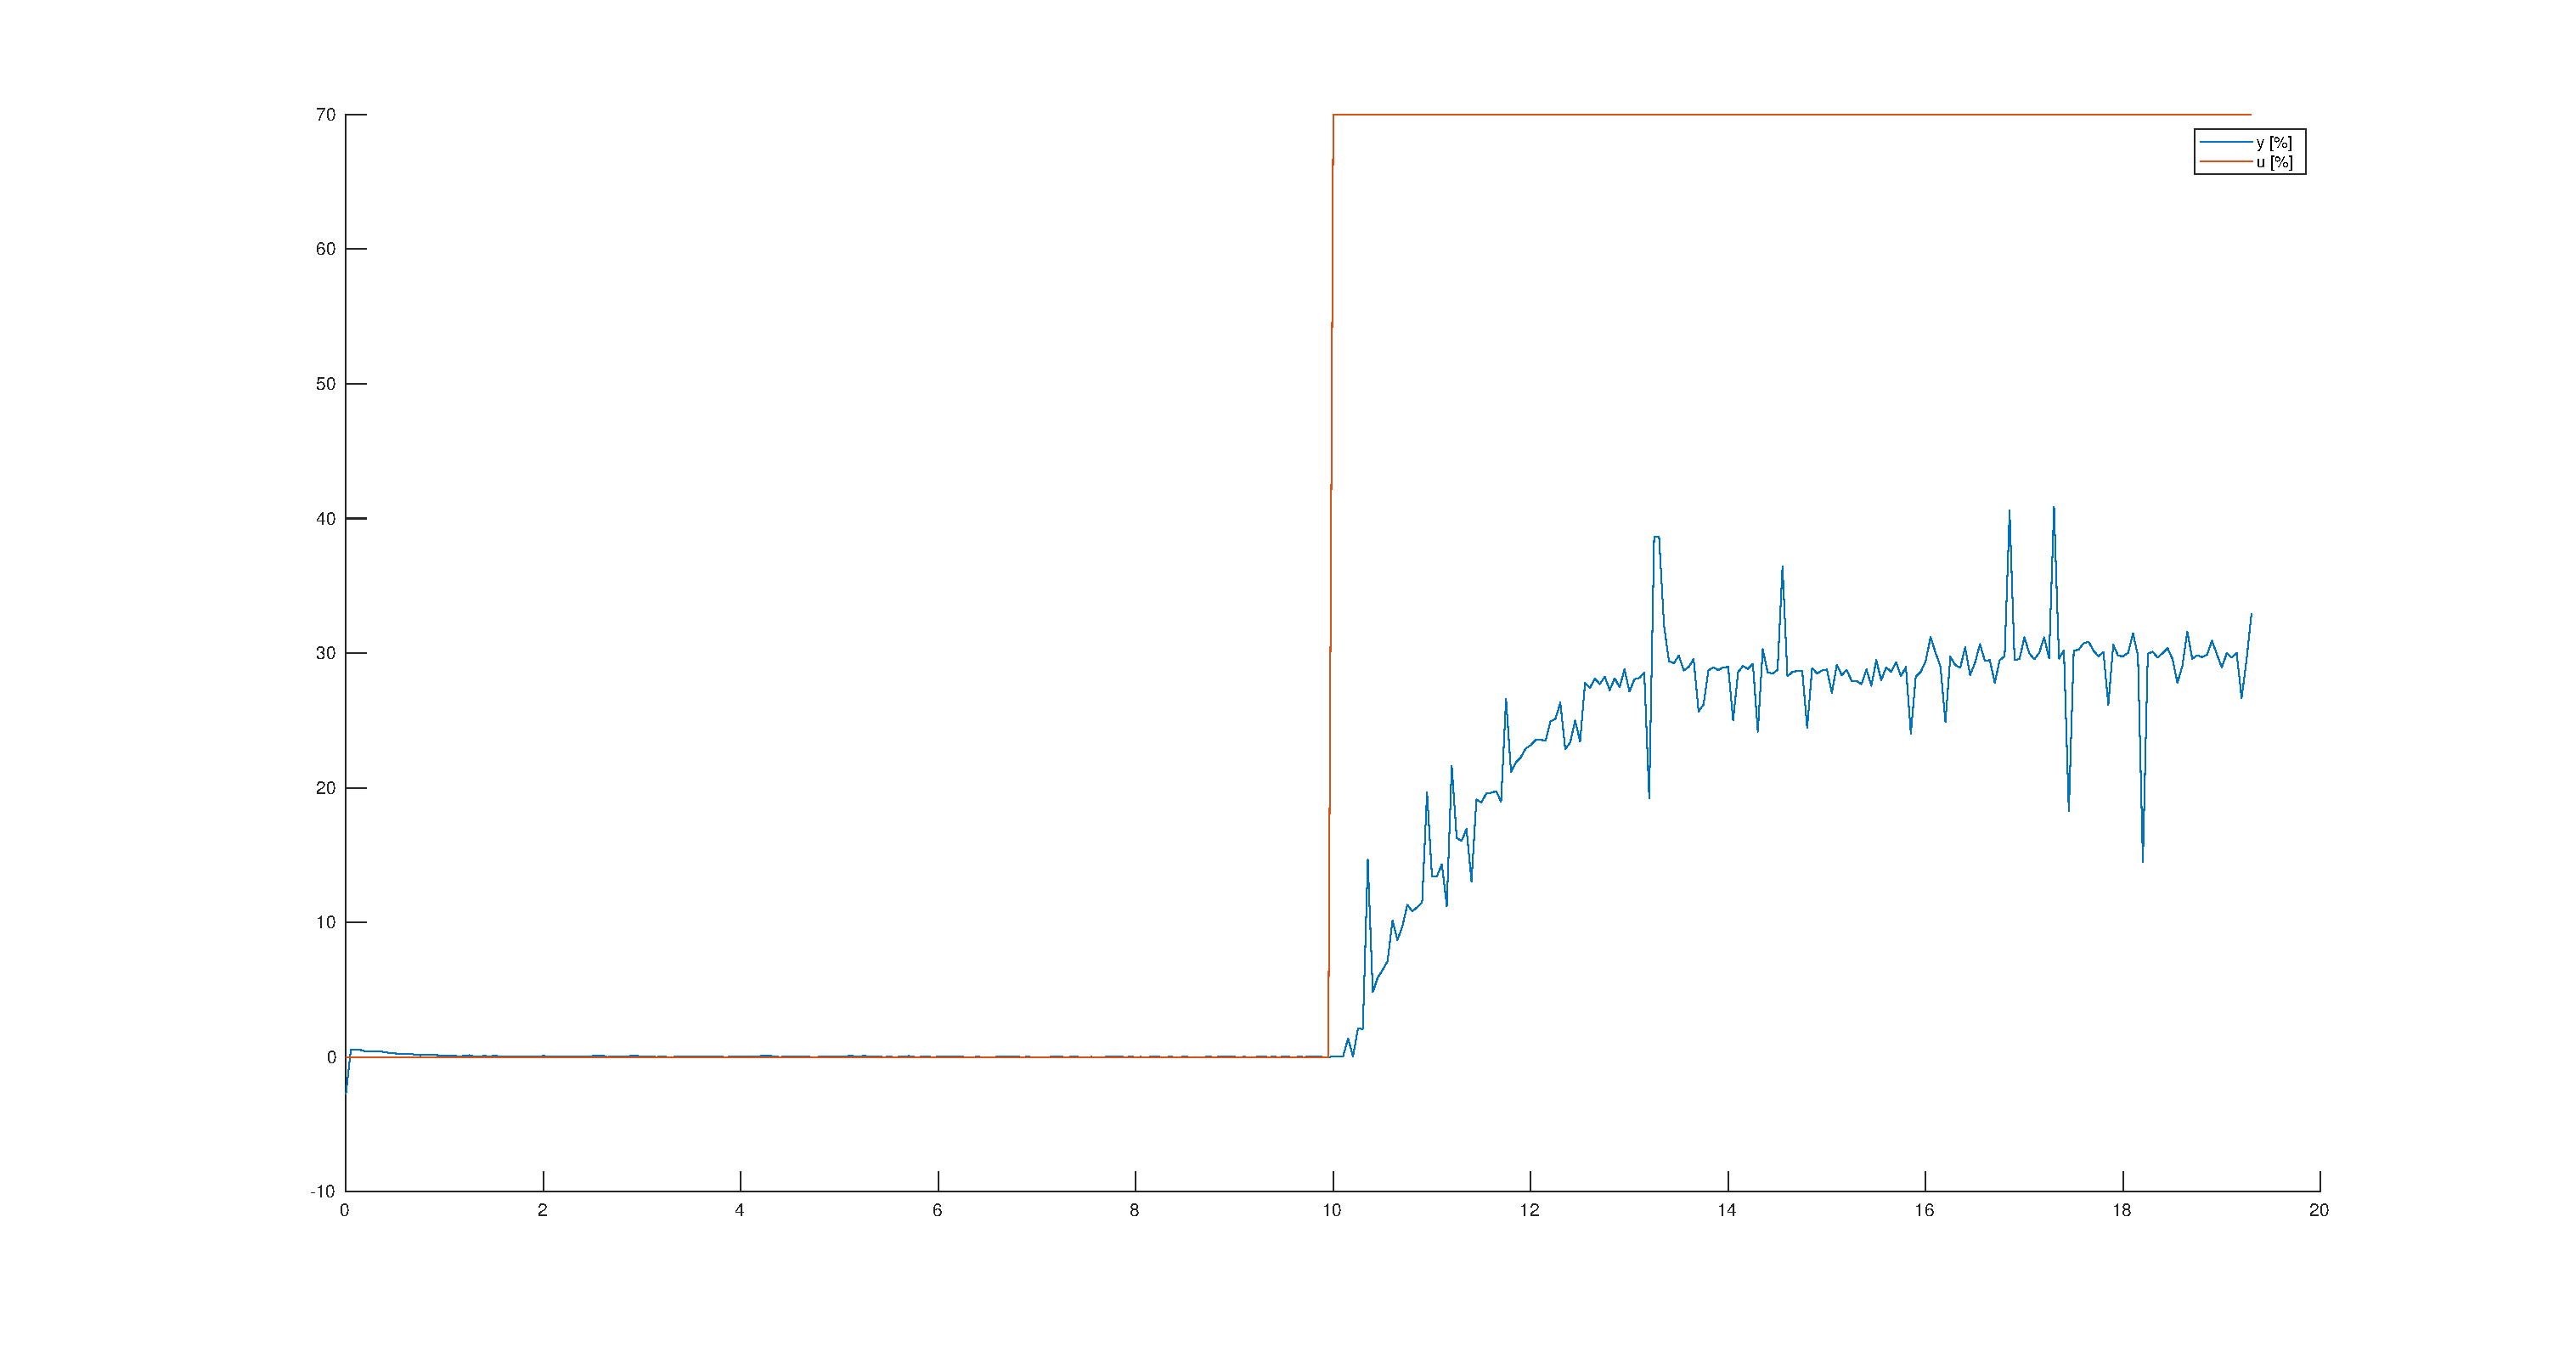
\includegraphics[width=1\textwidth]{1_3_1.eps}}
	\end{center}

\subsubsection {[1p] Comentarii referitor grafice obtinute }
\subsection {Datele masurate salvate }
\subsection {Caracteristici proces }
\begin{table}[H]
  \centering
  \begin{tabular}{|l|l|l|l|}
    \hline
    $t_c$ & $t_t$ & $\tau$ & $T_e\ ales$ \\
    \hline
    3.00 [s] & 3.2538 [s] & 0.2 [s] & 0.33 [s] \\
    \hline
  \end{tabular}
  \caption{Caracteristici proces alese experimental.}
\end{table}

\subsection {Rezolvare aplicatii laboratorul 3 }
Am ales urmatoarele proprietati pentru SPAB:
\begin{table}[h!]
  \centering
    \begin{tabular}{|l|l|l|l|}
      \hline
      $N$ & $p$ \\
      \hline
      9 & 2 \\
      \hline
    \end{tabular}
    \caption{Dataset description of the four datasets provided by Rabobank Group ICT.}
\end{table}

\begin{center}
  \fbox{ 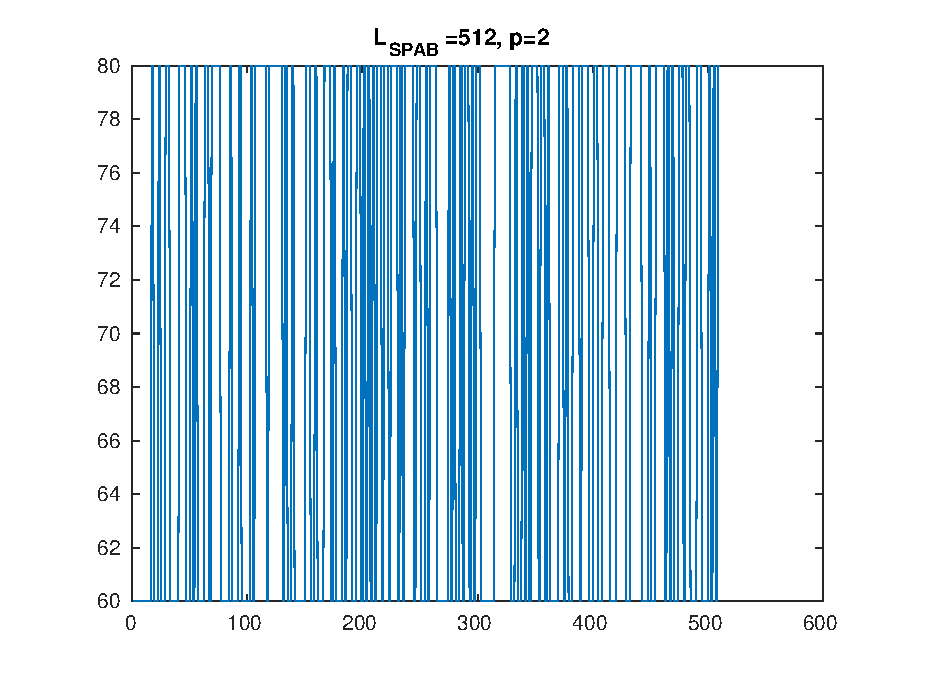
\includegraphics[width=0.8\textwidth]{1_6_1.eps}}
\end{center}

Algoritm generare SPAB:
\begin{lstlisting}
  uint32_t reg = 0b11111 1111; 

  int nr_val = 48; 

  for (int i = 0; i < nr_val; i++) { 
      std::cout << (reg & 1) << ", "; 
      uint8_t last_bit = !!((1 << 0) & reg) != !!((1 << 4) & reg); 
      reg >>= 1; 
      reg = reg | (last_bit << 8); 
  } 

  std::cout << std::endl;
\end{lstlisting}

Pentru vectorul initial:
\begin{lstlisting}
  0b11111'1111
\end{lstlisting}

Primele 48 valori:
\begin{lstlisting}
  1, 1, 1, 1, 1, 1, 1, 1, 1, 0, 0, 0, 0, 0, 1, 1, 1, 1, 0, 1, 1, 1, 1, 1, 0, 0, 0, 1, 0, 1, 1, 1, 0, 0, 1, 1, 0, 0, 1, 0, 0, 0, 0, 0, 1, 0, 0, 1
\end{lstlisting}

% Section 2
\section {Realizare si analiza experiment identificare }
\subsection {Expresia Matlab de generare a semnalului SPAB }
\begin{lstlisting}
  idinput(510, 'PRBS', [0 1/2], [6 8])
\end{lstlisting}

\subsection {[2p] Caracteristici semnal SPAB de intrare }
\begin{table}[H]
  \centering
  \begin{tabular}{|l|l|l|l|}
    \hline
    Tip semnal aleator & Lungime set date & Durata experiment & Banda de frecvente \\
    \hline
    SPAB & 762 & 251.46 [s] & [???] \\
    \hline
  \end{tabular}
  \caption{Caracteristici semnal SPAB}
\end{table}

\subsection {[3p] Afisare spectrul semnal SPAB de intrare }
\begin{center}
  \fbox{ 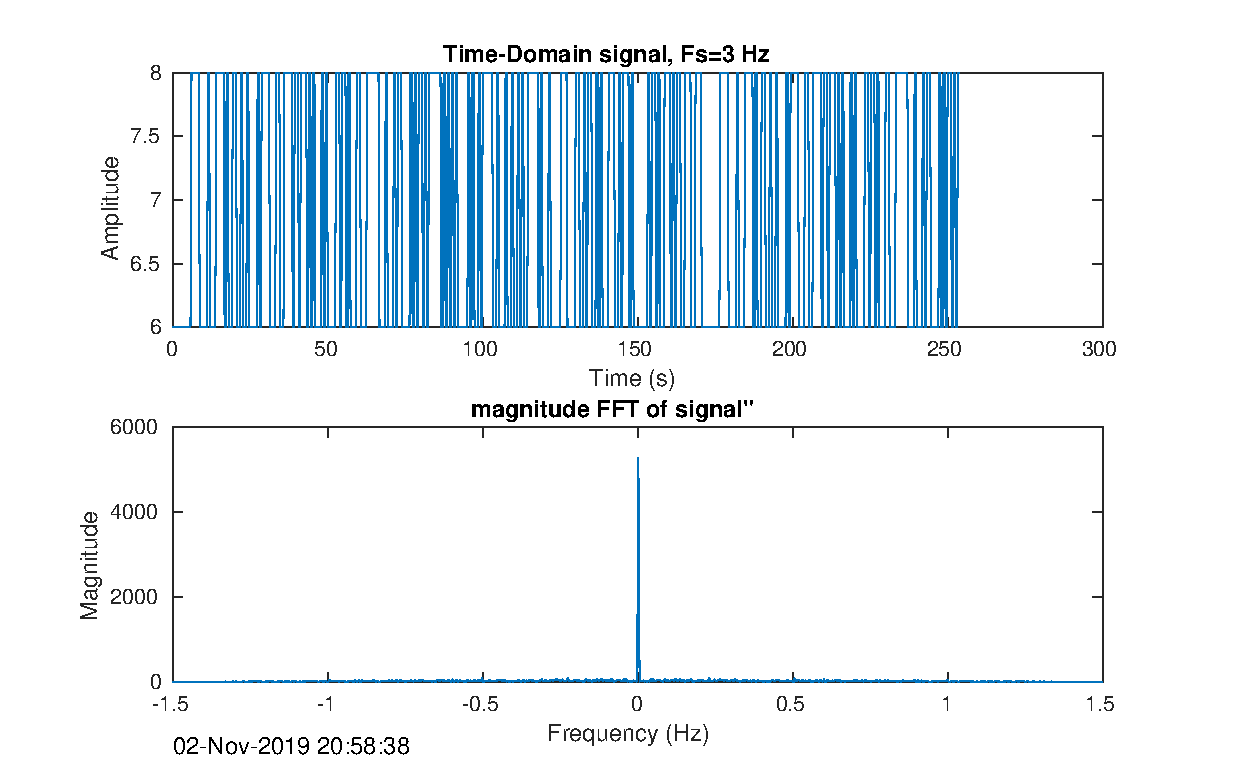
\includegraphics[width=0.8\textwidth]{2_3_1.eps}}
\end{center}

\subsection { [1p] Observatii asupra semnalului SPAB generat }
\subsection { Realizare experiment identificare (conform instructiunilor din laborator) }
Am realizat experimentul de identificare.
\subsection { Fisier rezultate identificare }
Numele fisierului este 'B70\_DateExper.mat'. Fiserul este de tip .mat in care este salvat o structura tip iddata care contine intrarea, iesirea si configurarea unor parametri (exp Te).
\subsection { [3p] Afisare spectrul semnal SPAB de iesire (achizitionat) }

\begin{center}
  \fbox{ 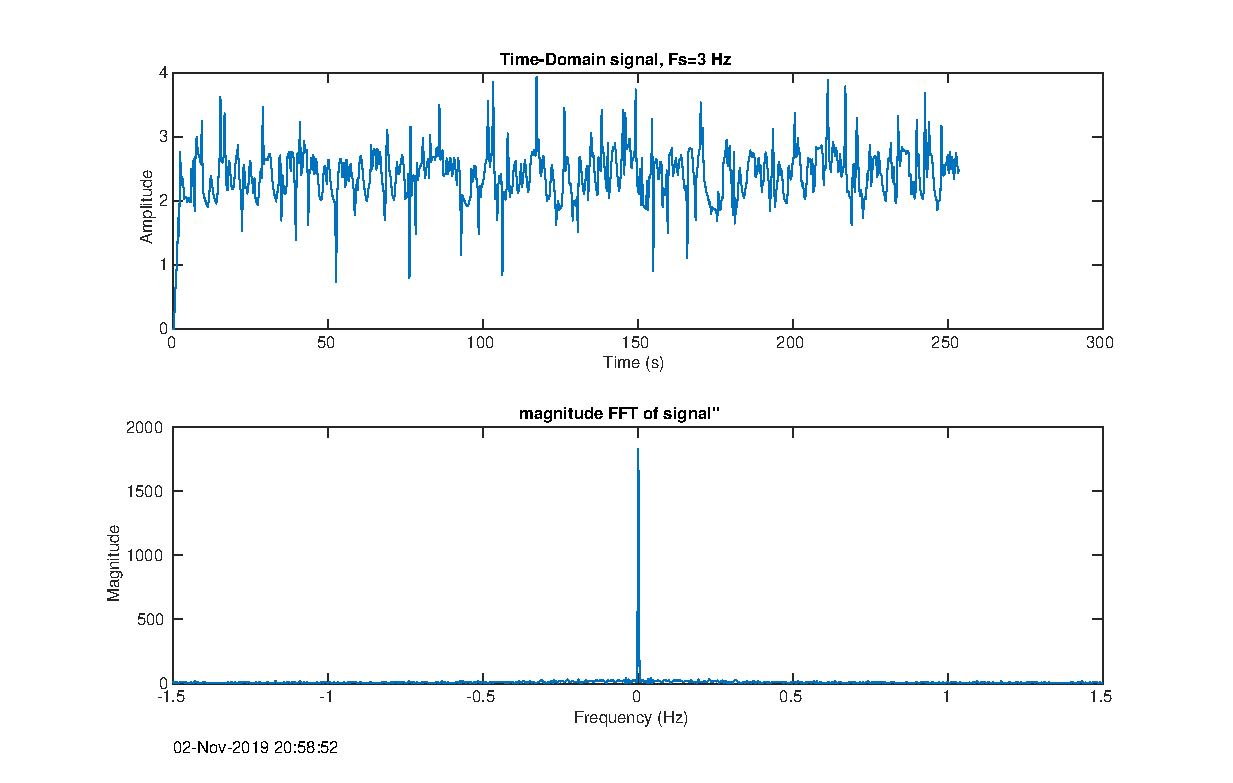
\includegraphics[width=0.8\textwidth]{2_7_1.eps}}
\end{center}

\subsection {[1p] Observatii asupra semnalului achizitonat }
Se observa favorizarea unor alte frecvente (in afara de 0Hz)

% Section 3
\section {IDENTIFICARE SI VALIDARE MODEL MATLAB }
\subsection {Platforma laborator 4 - citită}
\subsection {[2p+1p+2p] Rezolvare Aplicatii Lab 4 }
\subsubsection {Cum se determina daca un model este liniar sau neliniar?}
Se determina prin stimularea procesului cu diferite intrari de tip treapta pozitiva sau negativa de diferite amplitudini. Daca amplificarea statica a procesului $k_p = \dfrac{y_{stationar}}{u_{stationar}}$ are valori diferite, sau daca timpii de crestere sunt diferiti, atunci este vorba de un model neliniar

\subsubsection {Diferente intre ARIMAX si ARMAX}
Diferenta consta in filtrul perturbatiei $v$. Pentru modelul ARIMAX filtrul este $\dfrac{1}{C(q^-1)A(q^-1)}$, iar pentru ARMAX acesta este $\dfrac{C(q^-1)}{A(q^-1)}$.

\subsubsection {Intrebare pertinenta}
TO DO

\subsection {Filtrare semnale achiziționate in urma experimentului de identificare. }
\subsubsection {Functii Matlab apelate pentru filtrari: }
\begin{lstlisting}
  idata = iddata(data.IOData.signals(1).values, data.IOData.signals(2).values, 0.33)
  tr = getTrend(idata, 1)
  data_d = detrend(idata, tr);

  flt = butter(1, 0.2)
  flt_data = filter(flt(1), flt(2), data_d.OutputData)
  plotFreq(flt_data, 0.33)
\end{lstlisting}
\subsubsection {[2p] Spectru semnale filtrate: }
\begin{center}
  \fbox{ 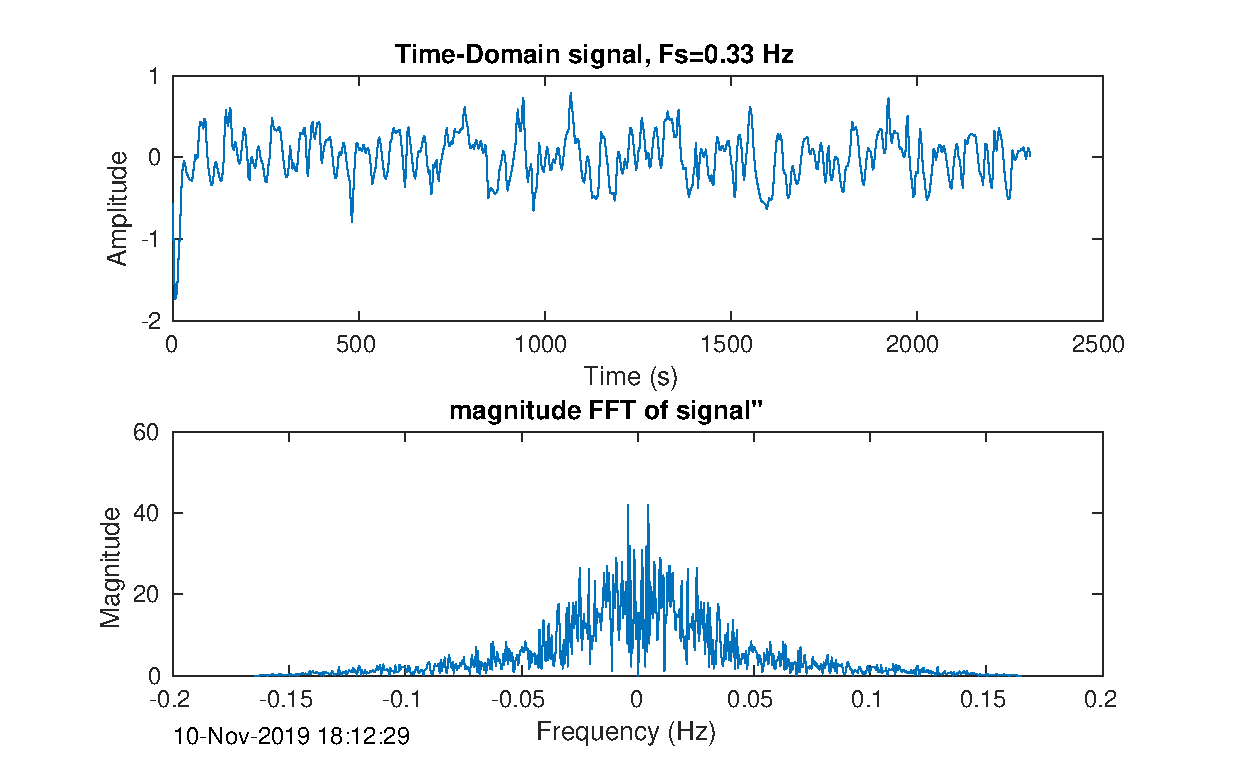
\includegraphics[width=0.8\textwidth]{3_3_2.eps}}
\end{center}
\subsubsection {[1p] Comentarii asupra spectrului }
TO DO - In esenta a disparut spike-ul
\subsection {Seturile de date de identificare Matlab - iddata pentru identificare si validare. }
\begin{lstlisting}
length(flt_data) % 762
eData = flt_data(1:508)
vData = flt_data(509:762)
\end{lstlisting}

\subsubsection {eData  (upload) }
\begin{lstlisting}
save(‘70BY_IdentData’,’eData’);
\end{lstlisting}
\subsubsection {vData  (upload) }
\begin{lstlisting}
save(‘70BY_ValidationData’,’vData’);
\end{lstlisting}
\subsection {[2p] Estimarea complexității model ARX }
\begin{lstlisting}
flt_idata = iddata(flt_data, data_d.InputData, 0.33)
e_idata = iddata(eData, data_d.InputData(1:508), 0.33)
v_idata = iddata(vData, data_d.InputData(509:762), 0.33)
\end{lstlisting}

\subsubsection {Utilizare functie advice: }
\begin{lstlisting}
General data characteristics:
-----------------------------
This is a time domain data set with 1 input(s) and 1 output(s),
254 samples and 1 experiment(s).

All inputs in the data have been denoted as 'zero order hold' ('zoh'), i.e. they are
assumed to be piecewise constant over the sample time.
If the input is a sampled continuous signal and you plan to build or convert to
continuous-time models, it is recommended to mark the InterSample property as
'First order hold': Data.InterSample = 'foh' or Data.int = {'foh','foh', ...} for
multi-input signals.


Some inputs and/or outputs have non-zero means. It is generally recommended to
remove the means by DAT = DETREND(DAT), except in the following cases:
1. The signals are measured relative to a level that corresponds to a
   physical equilibrium. This could e.g. be the case if step responses
   are recorded from an equilibrium point. In this case, it is advisable
   to remove the equilibrium values rather than data means. You may do so
   using a TrendInfo object with DETREND command, or during estimation using
   the "InputOffset" and "OutputOffset" estimation options.
2. There is an integrator in the system, and the input and output 
   levels are essential to describe the effect of the integration.
3. You are going to use the data to estimate nonlinear ARX models.

Excitation level in data:
-------------------------
The input is persistently exciting of order 50. This means that you
will encounter problems if estimating models of order higher than 50.

Possibility of feedback in data:
--------------------------------
There is a very strong indication of feedback in the data.
You should be careful when interpreting the results of SPA and also interpret
the results of output error models with care (Output error models result from
the OE command or setting 'DisturbanceModel'= 'None' in state-space models.).
With feedback in data, it is recommended to use estimate a model with large enough 
disturbance component. For example, use BJ models in place of OE models and estimate 
state space models using 'DisturbanceModel'= 'Estimate'. Also N4SID estimation using 
N4Weight = "SSARX" works better than other N4Weight options in handling data 
containing feedback.

Possibility of nonlinearity:
----------------------------
There is no clear indication of nonlinearities in this data set.
Use the "isnlarx" command to perform the assessment of nonlinearity with more options.
\end{lstlisting}

\subsubsection {Utilizare functie delayest: }
\begin{lstlisting}
ans =

     1
\end{lstlisting}

\subsubsection {Estimare complexitate model ARX }
\begin{table}[H]
  \centering
    \begin{tabular}{|l|l|l|l|}
      \hline
      $nA$ & $nB$ & $nk$ \\
      \hline
      -1 & -1 & -1 \\
      \hline
    \end{tabular}
    \caption{Caracteristici proces alese experimental.}
\end{table}

\subsection {Identificare model ARX }
\subsubsection {Descriere model obținut (structură, coeficienți, etc) }
\subsubsection {Valorile funcțiilor criteriu }
\subsubsection {Figurile obținute in urma validării ( resid \& compare) (vezi App Laborator 4) }
\subsection {[3p] Identificare model ARMAX }
\subsubsection {Descriere model obținut (structură, coeficienți, etc) }
\subsubsection {Valorile funcțiilor criteriu }
\subsubsection {Figurile obținute in urma validării ( resid \& compare) (vezi App Laborator 4) }
\subsection {[3p] Identificare model BJ }
\subsubsection {Descriere model ales (structură, coeficienți, etc) }
\subsubsection {Valorile funcțiilor criteriu }
\subsubsection {Figurile obținute in urma validării ( resid \& compare) (vezi App Laborator 4) }
\subsection {[3p] Identificare model OE }
\subsubsection {Descriere model ales (structură, coeficienți, etc) }
\subsubsection {Valorile funcțiilor criteriu }
\subsubsection {Figurile obținute in urma validării ( resid \& compare) (vezi App Laborator 4) }
\subsection {Alegere Model Final Matlab }
\subsubsection {Descriere model ales (structură, coeficienți, etc) }
\subsubsection {Valorile funcțiilor criteriu }
\subsubsection {Figurile obținute în urma validării (resid \& compare) }
\subsubsection {[1p] Studiul stabilității sistemului: ........... }
\subsubsection {Modelul Matlab ales încărcat este disponibil ?aici?. }
\subsubsection {Comentarii/Observații }

\section {MODELARE SI IDENTIFICARE FOLOSIND WIMPIM }
\subsection {4.1. [1p] Pregătire date inițiale WINPIM. Fisierul txt obtinut (upload) }
\subsection {4.2. [1p] Incarcare fisier in WinPIM si specificare perioada de esantionare }
\subsection {4.3. [1p] Aplicare filtrare set de date (eliminarea componentei continue) }
\subsection {4.4. [1p] Estimarea complexitatii}
\begin{table}[H]
  \centering
  \begin{tabular}{|l|l|l|l|}
    \hline
    $N$ & $n_A$ & $n_B$ & $d$ \\
    \hline
    0 & 0 & 0 & 0 \\
    \hline
  \end{tabular}
  \caption{Caracteristici proces alese experimental.}
\end{table}

\subsection {4.5. [5p]  Identificare si validare modele }
\subsection {4.6. [1p] Modelul ales este anexat aici (BXY.mod) }
\subsection {4.7. [2p] Simulare model ales WinPIM si simulare model ales Matlab. }
\subsection {4.8. [2p]  Graficele simularilor sunt disponibile aici .  }
\subsection {4.9. Modelul final ales pentru continuarea proiectului este: }

\section {CALCUL REGULATOR RST-1, SIMULARE SI VALIDARE }
a
\subsection {5.1. Platforma laborator 6 - citită }
\subsection {5.2.  Obiective de reglare impuse  : }
\subsection {5.3. Pulsatia naturala si atenuarea echivalente cu obiectivele de reglare impuse: }
\subsection {5.4.[2p] Polii dominanti discreti impusi ca urmare a obiectivelor de reglare: }
\subsection {5.5. [2p] Specificare polinom P: }
\subsection {5.6. [2p] Grade polinoame ecuatia Sylvester }
\subsection {5.7. [2p]  Matricea M asociata : }
\subsection {5.8. [1p] Solutia ecuatiei}
\subsection {5.9. [3p] Pentru ca sistemul sa ofere timp de raspuns minim si suprareglaj < 5\% se aleg: }
\subsection {5.10. [4p]  Simulare sistem in bucla inchisa (comanda, referinta, iesirea), in conditii de perturbatii treapta (25\% amplitudine) aplicate dupa stabilizarea sistemului fata de referinta. Graficele sunt prezentate aici: }
\subsection {5.11. [1p] Observatii legate de rezultatele obtinute: }
\subsection {5.12. [1p] Specificare polinom P: }
\subsection {5.13 [1p] Grade polinoame ecuatia Sylvester }
\subsection {5.14. [2p]  Matricea M asociata : }
\subsection {5.15. [1p] Solutia ecuatiei}
\subsection {5.16. [2p]  Simulare sistem in bucla inchisa (comanda, referinta, iesirea), in conditii de perturbatii treapta (25\% amplitudine) aplicate dupa stabilizarea sistemului fata de referinta. Graficele sunt prezentate aici: }
\subsection {5.17. [1p] Observatii legate de rezultatele obtinute: }

\section {PROIECTARE REGULATOR RST-1 - WINPIM }
a
\subsection {6.1. Specificare performante in urmarire respectiv in reglare: }
\subsection {6.2. Pentru regulatorul calculat folosind metoda Pole Placement, cu integrator, polinoamele R,S,T sunt: }
\subsection {6.3. Fisierul WinPim cu regulator si model este aici. }
\subsection {6.4. Simulare sistem in bucla inchisa (comanda, referinta, iesirea), in conditii de perturbatii treapta (25\% amplitudine) aplicate dupa stabilizarea sistemului fata de referinta. Graficele sunt prezentate aici: }
\subsection {6.5. Observatii legate de rezultatele obtinute: }

\section {EVALUARE EXPERIMENTALA REGULATOR RST-1 }
a
\subsection {7.1. Evaluare performante pe sistemul real. }
\subsubsection {Se alege referinta r(t) = a.i. u(t) stationar sa fie egal cu u0. Pentru aceasta referinta s-a stimulat sistemul si s-a aplicat si o perturbatie cand a ajuns in regimul stationar de cca.}
\subsubsection {Rezultatul simularii se afla in imaginea de mai jos: }
\subsubsection {[2p] Alegand o alta referinta raspunsul sistemului este capturat in figura de mai jos: }
\subsection {7.2. Performantele se regasesc rezumate in tabelul urmator }
\subsection {7.3. Comentarii privind calitatea solutiei obtinute vs specificatiile impuse: }

\section {CALCUL REGULATOR RST-2, SIMULARE SI VALIDARE }
a
\subsection {8.1. Platforma laborator 8 - citită }
\subsection {8.2. [2p] Regulatorul RST 1 si-a indeplinit sau nu performantele impuse ?  Daca nu, ce masuri se iau (ce specificatii noi se impun fata de primul design ) ? }
\subsection {8.3. [4p] Regulatorul RST 1 indeplineste marginile standard de robustete (se pot verifica cu aplicatia WinPIM)?   Figura cu functia de sensibilitate si template este furnizata aici. }
\subsection {8.4. [4p] In cazul in care regulatorul a trebuit recalculat acesta este descris de polinoamele: }
\subsection {8.5. [2p] Rezultatele in simulare sunt furnizate in figura urmatoare: }
\subsection {8.6. [2p] Functia de sensibilitate a noii solutii: }

\section {Evaluare Experimentala Regulator RST-2 }
a
\subsection {9.1. [3p] Evaluare performante pe sistemul real. }
\subsubsection {Se alege referinta r(t) = a.i. u(t) stationar sa fie egal cu u0. Pentru aceasta referinta s-a stimulat sistemul si s-a aplicat si o perturbatie cand a ajuns in regimul stationar de cca.\% }
\subsubsection {Rezultatul simularii se afla in imaginea de mai jos: }
\subsubsection {[2p] Alegand o alta referinta raspunsul sistemului este capturat in figura de mai jos: }
\subsection {9.2.[2p] Performantele se regasesc rezumate in tabelul urmator }
\subsection {9.3.[1p] Comentarii privind calitatea solutiei obtinute vs specificatiile impuse: }

\section {CONCLUZII GENERALE SI FEEDBACK PROIECT }
a
\subsection {Concluzii legate de solutia de reglare calculata }
\subsection {Feedback legat de desfasurare/ continut proiect }

\end{document}
